\documentclass[10pt,a4paper]{article}
\usepackage[utf8]{inputenc}
\usepackage[finnish]{babel}
\usepackage[T1]{fontenc}
\usepackage{amsmath}
\usepackage{amsfonts}
\usepackage{amssymb}
\usepackage{hyperref} % Add a link to your document
\usepackage{graphicx} % Add pictures to your document
\usepackage{listings} % Source code formatting and highlighting
\pagenumbering{arabic}

\begin{document}
\author{Ville-Veikko Saari}
\title{Discgolf scorekeeper - Fisbeegolf pistetilasto}
\maketitle
\newpage
\tableofcontents
\newpage
\section{Johdanto}
Tavoitteena on toteutta frisbeegolffia varten pistetilastointijärjestelmä, joka voisi olla myös laajennettavissa erilaisille mobiilialustoille. Lähtökohtaisesti tarkoituksena on kuitenkin rakentaa tietokanta johon voi lisätä tulokset jälkeenpäin ja selata aiempia tilastoja.
\subsection{Järjestelmän tarkoitus}
Järjestelmän tarkoituksena on helpottaa frisbeegolfin pelaajia omien ja ystävien suoritusten seuraamisessa eri radoilla, sekä säilöä niitä myöhempää vertailua varten.
\subsection{Järjestelmän toteutus}
Toteutus tapahtuu Postgres-tietokantaa käyttävänä PHP-sovelluksena johon on pääsy tavallisella verkkoselaimella. Työ sijaitsee ainakin aluksi Helsingin Yliopiston Tietojenkäsittelytieteen laitoksen users-palvelimella jossa palvelinsovelluksena toimii Apache.
\newpage
\section{Yleiskuva järjestelmästä}

\subsection{Käyttötapauskaavio}
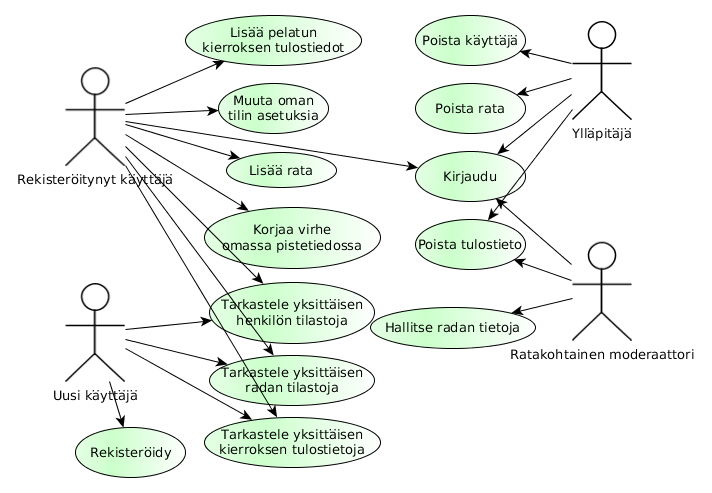
\includegraphics[scale=0.5]{kayttotapauskaavio}

\subsection{Käyttäjäryhmät}
\textbf{Ylläpitäjä} on sivuston vahtikoira. Hänen tehtävä on vahtia sisältöä ja siivota tarvittaessa roskadataa pois. Ylläpitäjä on myös palvelun ylin muokkaaja, joka voi muunmuassa yhdistää kaksi tai useampaa samaa rataa yhdeksi.

\noindent\textbf{Ratakohtainen moderaattori} toimii hieman kuten ylläpitäjä, mutta yksittäisen radan kontekstissa. Lähtökohtaisesti ratakohtainen moderaattori on radan luonut henkilö tai tämän henkilön astuessa tehtävästä sivuun, jokin toinen käyttäjä.

\noindent\textbf{Rekisteröitynyt} käyttäjä on käyttäjä joka on luonut tilin palveluun.

\noindent\textbf{Uusi käyttäjä} on käyttäjä jolla ei ainakaan vielä ole tiliä palveluun.

\subsection{Käyttötapauskuvaukset}
\paragraph{Ylläpitäjä} \hspace{0pt}
\\\textbf{Kirjaudu:} Ylläpitäjän täytyy kirjautua sisään palveluun tunnuksella ja salasanalla ennen kuin voi tehdä mitään ylläpitäjän toimista.
\\\textbf{Poista käyttäjä:} Ylläpitäjä voi poistaa häiritsevän käyttäjän tarvittaessa. Poistaminen ei varsinaisesti poista kaikkea käyttäjään liittyvää tietoa ainakaan heti, vaan laittaa käyttäjän jonkinlaiseen estettyyn tilaan.
\\\textbf{Poista rata:} Ylläpitäjä voi poistaa radan tai yhdistää sen jo olemassa olevaan.
\\\textbf{Poista tulostieto:} Ylläpitäjä voi poistaa tulostiedon tarvittaessa.
\paragraph{Ratakohtainen moderaattori} \hspace{0pt}
\\\textbf{Kirjaudu:} Moderaattorin täytyy kirjautua sisään palveluun tunnuksella ja salasanalla ennen kuin voi tehdä mitään moderaattorin toimista.
\\\textbf{Hallitse radan tietoja:} Moderaattori voi kirjoittaa radalle kuvauksen ja lisätä esimerkiksi radan väylätiedot, kartan radasta, sekä linkin sen sijaintiin karttapalvelussa.
\\\textbf{Poista tulostieto:} Moderaattori voi poistaa tulostiedon tarvittaessa.
\paragraph{Rekisteröitynyt käyttäjä} \hspace{0pt}
\\\textbf{Kirjaudu:} Käyttäjän täytyy kirjautua sisään palveluun tunnuksella ja salasanalla ennen kuin voi tehdä mitään rekisteröityneille käyttäjille rajoitetuista toimista.
\\\textbf{Muuta oman tilin asetuksia:} Käyttäjä voi muokata omia tietojaan.
\\\textbf{Lisää pelatun kierroksen tulostiedot:} Käyttäjä voi lisätä radan alle tulostiedot pelaamastaan kierroksesta.
\\\textbf{Korjaa virhe omissa tulostiedoissa:} Käyttäjä voi jälkeenpäin muokata lisäämäänsä tulostietoa.
\\\textbf{Lisää rata:} Jos rataa ei vielä löydy palvelusta, käyttäjä voi lisätä sen. Samalla hänestä tehdään myös kyseisen radan moderaattori kunnes hän antaa kyseisen toimen toiselle käyttäjälle tai on pitkään tekemättä tarvittavia toimenpiteitä radan sivulla.
\paragraph{Uusi käyttäjä} \hspace{0pt}
\\\textbf{Rekisteröidy:} Uusi käyttäjä voi rekisteröityä saadakseen käyttöönsä laajemmat toiminnallisuudet.
\\\textbf{Tarkastele yksittäisen henkilön tilastoja:} Kuka tahansa voi katsoa yksittäisen henkilön tulostilastoja.
\\\textbf{Tarkastele yksittäisen radan tilastoja:} Kuka tahansa voi katsoa yksittäisen radan tulostilastoja.
\\\textbf{Tarkastele yksittäisen kierroksen tilastoja:} Kuka tahansa voi katsoa yksittäisen kierroksen tulostilastoja.


\newpage
\section{Järjestelmän tietosisältö}
\subsection{Tietosisällön käsitekaavio}
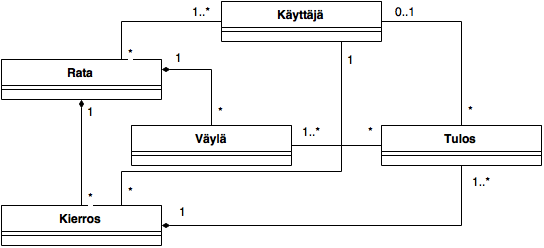
\includegraphics[scale=0.6]{tsoha_tietosisalto}
\subsection{Tietokohteet}
\subsubsection{Käyttäjä}
    \begin{tabular}{ | l | p{3cm} | p{5cm} |}
    \hline
    Attribuutti & Arvojoukko & Kuvailu\\ \hline
    nimi & Merkkijono, max. 50 merkkiä & Käyttäjän koko nimi. \\ \hline
    kotirata & integer & Kotiradan id. \\ \hline
    tunnus & Merkkijono, max. 15 merkkiä & Käyttäjän tunnus. \\ \hline
    salasana & Binääri & Salasanan tiiviste ja suola. \\ \hline
    ylläpitäjä & Boolean & Tosi, jos käyttäjä on ylläpitäjä \\ \hline
    \end{tabular}\\
Käyttäjään voi liittyä useita muita käyttäjiä ns. seurattujen käyttäjien tai kaverilistan muodossa. Käyttäjään voi liittyä useita tuloksia. Lisäksi käyttäjällä voi olla useita ratoja moderoitavanaan.
\subsubsection{Rata}
    \begin{tabular}{ | l | p{3cm} | p{5cm} |}
    \hline
    Attribuutti & Arvojoukko & Kuvailu\\ \hline
    nimi & Merkkijono, max. 100 merkkiä & Radan nimi. \\ \hline
    sijainti & Merkkijono, max. 300 merkkiä & Radan osoite. \\ \hline
    karttalinkki & Merkkijono, max. 300 merkkiä & Linkki radan sijaintiin karttapalvelussa. \\ \hline
    kuvaus & Merkkijono, max. 500 merkkiä & Kuvaus radasta. \\ \hline
    \end{tabular}\\
Rataan liittyy vähintään yksi moderaattori. Moderaattoriksi määritellään aluksi käyttäjä joka radan lisää palveluun. Rataan kuuluu myös väyliä ja kierroksia.
\subsubsection{Väylä}
    \begin{tabular}{ | l | p{3cm} | p{5cm} |}
    \hline
    Attribuutti & Arvojoukko & Kuvailu\\ \hline
    rata & integer & Radan, johon väylä kuuluu, id. \\ \hline
    nimi & Merkkijono, max. 100 merkkiä & Väylän mahdollinen nimi, voi olla myös tyhjä. \\ \hline
    par & integer & Väylän ihann	etulos. \\ \hline
    väylänumero & integer & Monesko väylä radalla. \\ \hline
    käytössä & Boolean & Tosi, jos väylä on edelleen käytössä. \\ \hline
    \end{tabular}\\
Väylä liittyy aina johonkin rataan ja tietää itse monesko väylä radalla on. Tuloksen ja väylän välillä on yhteys, jotta tulos tietää mikä on väylän ihannetulos.
\subsubsection{Kierros}
    \begin{tabular}{ | l | p{3cm} | p{5cm} |}
    \hline
    Attribuutti & Arvojoukko & Kuvailu\\ \hline
    rata & integer & Radan, jolla kierros pelattiin, id. \\ \hline
    ajankohta & Datetime & Kierroksen aloitusajankohta. \\ \hline
    käyttäjä & integer & Kierroksen lisänneen käyttäjän id. \\ \hline
    \end{tabular}\\
Kierros liittyy aina rataan ja kierrokseen liittyy yksi tai useampi tulos, riippuen siitä montako pelaajaa kierroksella on ollut. Kierros on itsessään kuvaus tapahtuneesta pelikierroksesta kyseisellä radalla.
\subsubsection{Tulos}
    \begin{tabular}{ | l | p{3cm} | p{5cm} |}
    \hline
    Attribuutti & Arvojoukko & Kuvailu\\ \hline
    kierros & integer & Kierroksen, jolta tulos on, id. \\ \hline
    käyttäjä & integer & Käyttäjän, jota tulos koskee, id. \\ \hline
    nimi & Merkkijono, max. 50 merkkiä & Jos pelaaja ei ole vielä käyttäjä, voidaan antaa merkkijonona nimi pelaajalle. \\ \hline
    \end{tabular}\\
Tulos on yhden pelaajan tulos. Käyttäjä kenttä voi olla tyhjä, jos pelaaja ei ole käyttäjä. Tulos tietää miltä väylältä tulos on, ja varsinainen numeerinen heittojen määrä tallennetaankin tuloksen ja väylän väliseen liitostauluun.
\newpage
\section{Relaatiotietokanta}
\subsection{Relaatiotietokantakaavio}
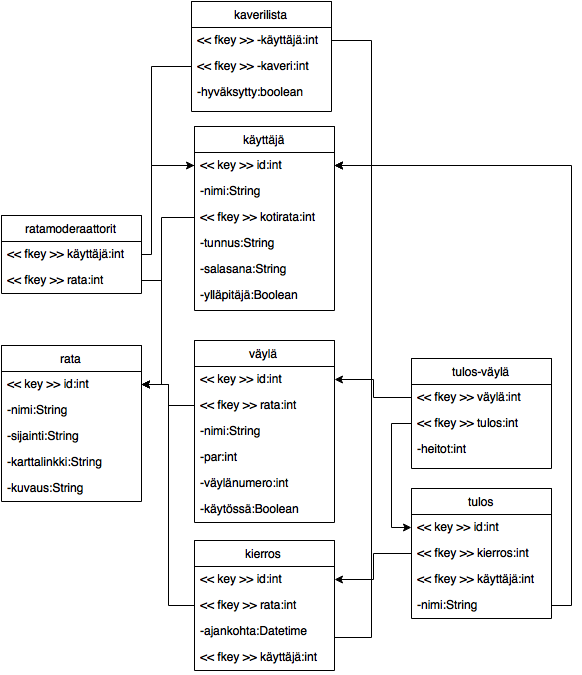
\includegraphics[scale=0.6]{tsoha_relaatiotietokantakaavio	}
\end{document}